\section{Controles}

\begin{figure}[htbp]
\begin{center}
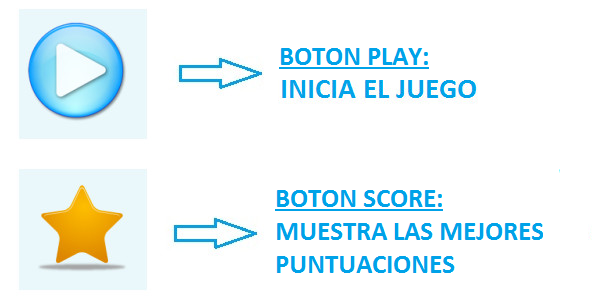
\includegraphics[width=.40\textwidth]{./imagenes/Controles.png}
\caption{Controles}
\label{Controles}
\end{center}
\end{figure}


\begin{center}
\textbf{NUEVO JUEGO} 
\\ Inicia una nueva partida en cualquier instancia del Juego.
\ \\ \ \\

\textbf{BORRAR JUEGO} 
\\ Elimina el contenido de todas las casillas. \ \\ \ \\

\textbf{COMPROBAR} 
\\ Verifica si la solución propuesta por el usuario esta correcta o incorrecta. 
\ \\ \ \\

\textbf{RESOLVER JUEGO}  
\\ Muestra la solución del SUDOKU. 
\ \\ \ \\

\textbf{SALIR}  
\\ Cierra la aplicación. 
\ \\ \ \\ 

\textbf{GUARDAR PARTIDA}  
\\ Guarda una partida iniciada. 
\ \\ \ \\ 

\textbf{CARGAR PARTIDA}  
\\ Carga una partida que ha sido guardada. 
\ \\ \ \\ 

\textbf{ALERTA DE JUGADAS INVALIDAS}  
\\ Muestra una alerta cuando se digita un valor incorrecto en alguna casilla. 
\ \\ \ \\ 

\textbf{ALERTA DE JUGADAS INCORRECTAS}  
\\ Muestra una alerta en todas las casillas que tienen valores incorrectos. 
\ \\ \ \\ 

\textbf{SCORE DE PARTIDAS}  
\\ Visualiza las mejores partidas. 
\ \\ \ \\ 

\textbf{DIFICULTAD} 
\\ Consta de 3 niveles.
\end{center}

\begin{figure}[htbp]
\begin{center}
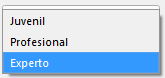
\includegraphics[width=.20\textwidth]{./imagenes/Nivel.png}
\caption{Niveles de Dificulatad}
\label{Niveles de Dificulatad}
\end{center}
\end{figure}

\begin{center}
Seleccionando la opción \textbf{MENU -> QUIT} (Figura 5.5) también podemos cerrar la aplicación y al seleccionar la opción \textbf{ACERCA DE.. -> HELP} (Figura 5.6) obtenemos información de la aplicación.
\end{center}

\begin{figure}[htbp]
\begin{center}
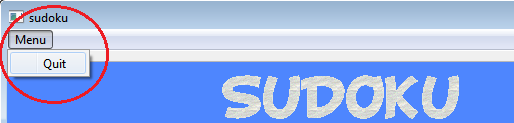
\includegraphics[width=.15\textwidth]{./imagenes/SeleccionMenu.png}
\caption{Opción Menu}
\label{Opcion Menu}
\end{center}
\end{figure}

\begin{figure}[htbp]
\begin{center}
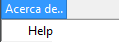
\includegraphics[width=.15\textwidth]{./imagenes/SeleccionAcerca.png}
\caption{Opción Acerca de..}
\label{Opcion Acerca de..}
\end{center}
\end{figure}




